\chapter{Antecedentes}

En este capítulo se expondrán los fundamentos teóricos y conceptuales necesarios en el desarrollo del proyecto. Se abordarán los principales conceptos y características de las antenas, teniendo en cuenta que por naturaleza un radiotelescopio es una antena. Además, se explicará el funcionamiento de los receptores heterodinos, principal componente utilizado en la digitalización y adquisición de señales de RF. Para finalmente, abordar el concepto de radiotelescopio, la importancia de la línea de Hidrógeno neutro y el proyecto CHARTS.\\

\section{Fundamentos de antenas}

Una antena es un dispositivo usualmente pasivo que convierte radiación electromagnética del ambiente en corriente eléctrica y viceversa, dependiendo para qué se utilice, pueden ser configuradas para recibir o transmitir señales. Los radiotelescopios son antenas receptoras. Suele ser fácil calcular las propiedades de una antena transmisora y medir las propiedades de una antena receptora. Afortunadamente, la mayor parte de las propiedades de una antena transmisora (como el patrón de radiación) son equivalentes al usar esta misma antena como receptora, así como cualquier medición de una antena receptora puede ser aplicada a esta antena cuando es usada para la transmisión \cite{Ransom2016}.\\

\subsection{Patrón de radiación}

El patrón de radiación es una representación gráfica de las propiedades radiativas de una antena. Se define como el gráfico de potencia transmitida por la antena, evaluada sobre una esfera de radio constante. Por razones prácticas se estudian cortes del patrón de radiación. Estos cortes son las curvas tridimensionales del patrón que son contenidas en la intersección de la esfera pasando por el origen.\\

Para poder medir la potencia radiada por una antena, se debe obtener utilizando la aproximación de campo lejano. El campo lejano es la distancia donde debe encontrarse una fuente puntual para que sus ondas recibidas sean planas \cite{Ransom2016}. Lo que en consecuencia significa que la radiación se propaga en modo TEM, es decir, que la componente eléctrica es perpendicular a la componente magnética y ambas son perpendiculares a la dirección de propagación, esto permite solo utilizar el campo eléctrico para describir la radiación \cite{Astudillo2014}.\\

\subsubsection*{Campo Lejano} La definición de la distancia de campo lejano depende tanto de la longitud de onda $\lambda$ como el tamaño de la antena $D$, o diámetro para antenas de apertura parabólicas. La distancia de campo lejano se define como:

\begin{equation}
    R = \frac{2D^2}{\lambda}
\end{equation}

Se utiliza las definiciones de campo eléctrico normalizado y potencia normalizada para poder expresar el patrón de radiación en decibelios. Utilizando el máximo como el valor de referencia. La potencia normalizada se define como:\\

\begin{equation}
    \Vec{F}(\theta, \Phi)=\frac{\Vec{E(\theta, \phi)}}{max|\Vec{E}(\theta, \phi)|}
\end{equation}

\begin{equation}
    P(\theta, \phi) = |\Vec{F}(\theta, \phi)|^{2}
\end{equation}

\begin{equation}
    P(\theta, \phi)_{dB} = 10logP(\theta, \phi)=20log |\Vec{F}|=F(\theta, \phi)
\end{equation}


\begin{figure}
    \centering
    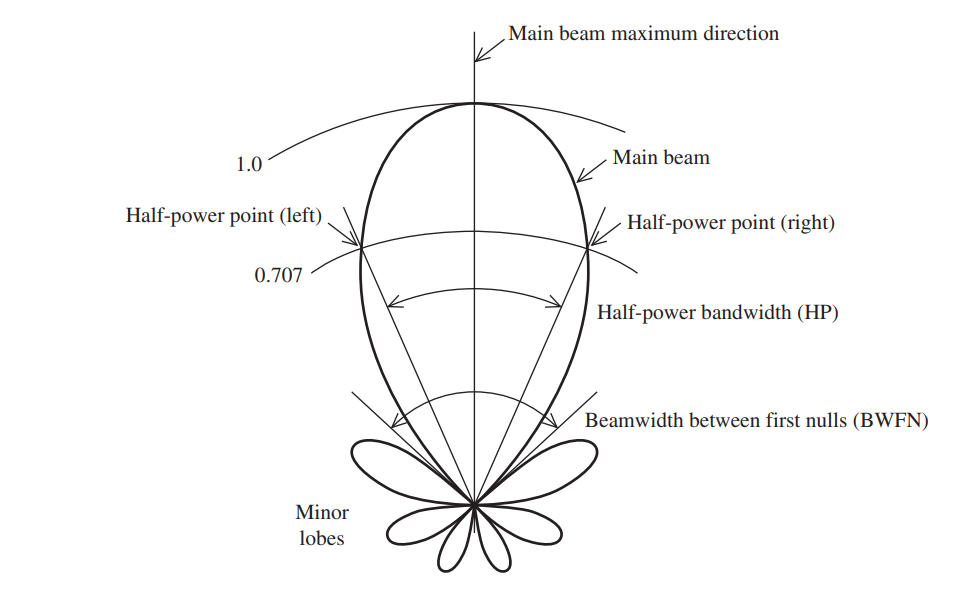
\includegraphics[width = 11cm]{img/patern1.png}
    \caption{Parámetros del patrón de radiación para una antena con características directivas. \cite{stutzman2012antenna}.}
    \label{fig:patern}
\end{figure}

La figura \ref{fig:patern}, muestra un patrón de radiación de una antena directiva, donde se pueden observar los lóbulos laterales y el haz principal. El haz principal es la dirección de máxima radiación, mientras que los lóbulos laterales son las direcciones de radiación secundarias.\\

El haz principal se define en términos de potencia y se conoce como HPBW o Haz de Media Potencia. El HPBW es el ángulo entre los puntos de la curva de radiación que tienen la mitad de la potencia máxima, es decir donde se ve una disminución de 3 dB.\\

\subsection{Directividad}

La directividad (D) se define como la razón de intensidad de radiación en una dirección específica con respecto a la intensidad promedio de radiación en todas las direcciones. Esta referencia se toma desde el máximo de radiación.\\

\begin{equation}\label{eq:directivity}
    D = \frac{U(\theta, \phi)}{U_{prom}}
\end{equation}

Donde $U(\theta, \phi)$ es la densidad de potencia radiada en una dirección específica y $U_{prom}$ es la densidad de potencia promedio. Lo que da a entender que la directividad es comúnmente adimensional.\\

La directividad se puede expresar directamente del patrón de radiación de la antena. Para esto se define un haz de ángulo sólido $d\Omega$  y se integra sobre la superficie de una esfera de radio R.\\

\begin{equation}\label{eq:solidangle}
    \Omega_{A} = \int\int_{esfera} |F(\theta, \phi)|^{2} d\Omega
\end{equation}

El ángulo sólido de un haz de un patrón de radiación tiene el mismo máximo de intensidad de radiación que toda el área del ángulo sólido del haz.\\

\begin{equation}\label{eq:powerdensity}
    P = U_{prom} \Omega_{A}
\end{equation}

Finalmente, si se reemplaza la ecuación \ref{eq:solidangle} en la ecuación \ref{eq:powerdensity} se obtiene la directividad de la antena a partir del ángulo sólido del haz del patrón de radiación.\\

\begin{equation}
    D = \frac{4\pi}{\Omega_{A}}
\end{equation}

Esto quiere decir que la directividad está completamente definida por la forma del patrón de radiación. Haciendo que sea totalmente independiente de la construcción de la antena \cite{stutzman2012antenna}.\\


\subsection{Ganancia}

La ganancia de una antena se define como la potencia transmitida en una dirección específica con respecto a la potencia transmitida por una antena isotrópica. La ganancia se define como:

\begin{equation}
    G = \frac{4\pi U_{m}}{P_{in}}
\end{equation}

Donde $U_{m}$ es la densidad de potencia máxima y $P_{in}$ es la potencia de entrada a la antena. La ganancia también se puede representar como la directividad multiplicada por la eficiencia de la antena.\\

\begin{equation}
    G = \varepsilon D 
\end{equation}

La eficiencia de una antena se define como la razón de la potencia radiada por la antena a la potencia total suministrada a la antena.\\

\begin{equation}
    \varepsilon = \frac{P_{rad}}{P_{in}}
\end{equation}

En el caso particular de una antena de apertura, el término de la eficiencia también incluye factores como la iluminación de la antena y las pérdidas de la superficie, las cuales se denominan eficiencia de apertura y eficiencia de superficie respectivamente.\\

\begin{equation}
    \varepsilon_{ap} = e_{r} \varepsilon_{t} \varepsilon_{s} \varepsilon_{a}
\end{equation}

Donde $e_{r}$ es la eficiencia de la radiación, $\varepsilon_{t}$ es la eficiencia \textit{taper} o de cobertura, $\varepsilon_{s}$ de \textit{spillover} o de derrame e $\varepsilon_{a}$ es la eficiencia de \textit{achivement} o de completitud, la cual incluye muchas otras fuentes de pérdidas.\\

Así, la ganancia de una antena de apertura es directamente proporcional a su apertura física y a la longitud de onda de la señal que se desea recibir.\\

\begin{equation}
    G = \frac{4\pi A}{\lambda^{2}} = \varepsilon_{ap} D
\end{equation}

$A$ es el área de la apertura de la antena y $\lambda$ es la longitud de onda.\\

\subsection{Polarización}

La polarización de una antena es la polarización de la onda electromagnética irradiada en una dirección dada por la antena al transmitir. Se describe como la orientación del campo eléctrico de la onda.\\

\begin{figure}
    \centering
    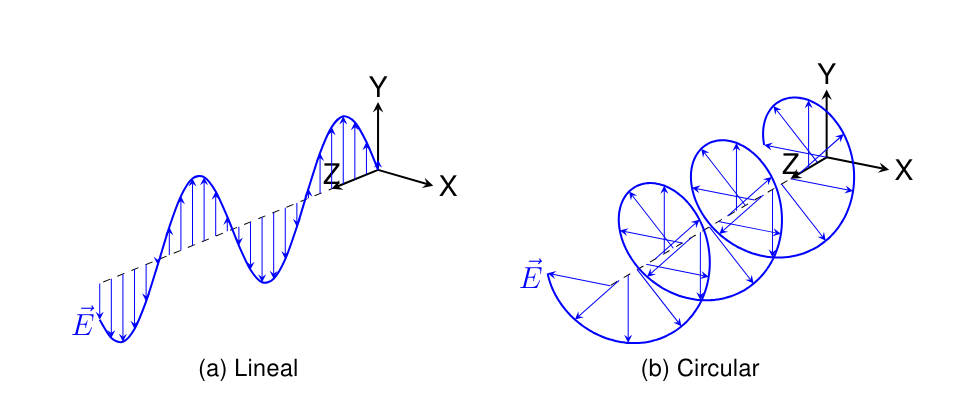
\includegraphics[width = 0.8\linewidth]{img/pol}
    \caption{Polarización linear y circular de una onda electromagnética propagándose en el eje Z.}
    \label{fig:polarizacion2}
\end{figure}

Los tipos de polarización se dividen en polarización lineal, polarización circular y la combinación de ambas, la polarización elíptica. La figura 2.2a muestra una onda electromagnética linealmente polarizada en orientación vertical. La figura 2.2b muestra una onda electromagnética circularmente polarizada en sentido horario.\\



\subsection{Ancho de banda}

El rango de frecuencia en el cual una antena opera con su mejor eficiencia se le denomina como ancho de banda. El ancho de banda se define considerando los parámetros de reflexión y de radiación de potencia, siendo comúnmente utilizados los parámetros de reflexión $S_{11}$ y transmisión $S_{21}$ para esta caracterización.\\

Los parámetros S son los que definen la respuesta de un medio a una onda electromagnética. Existen los parámetros $S_{11}$, $S_{12}$, $S_{21}$ y $S_{22}$, donde $S_{11}$ es el parámetro de reflexión, $S_{12}$ es el parámetro de transmisión, $S_{21}$ es el parámetro de transmisión inversa y $S_{22}$ es el parámetro de reflexión inversa.\\

\begin{figure}
    \centering
    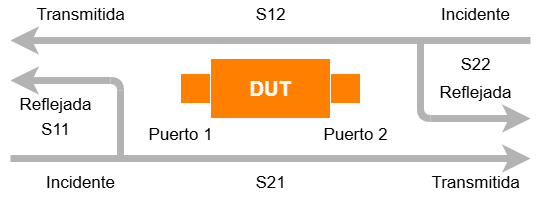
\includegraphics[width = 0.8\textwidth]{img/bloquesS.png}
    \caption{Diagrama de parámetros S para un dispositivo bajo prueba (DUT).}
    \label{fig:sparam}
\end{figure}

La figura \ref{fig:sparam} muestra las diferentes configuraciones para lograr la obtención de los parámetros S.\\

\paragraph{Ancho de banda $S_{11}$} El ancho de banda de reflexión se define como el rango de frecuencia en el cual el parámetro de reflexión $S_{11}$ es menor a un valor específico, comúnmente -10 dB. Lo que corresponde a que el 90\% de la potencia inyectada es irradiada y solo el 10\% reflejada\\

\begin{figure}
    \centering
    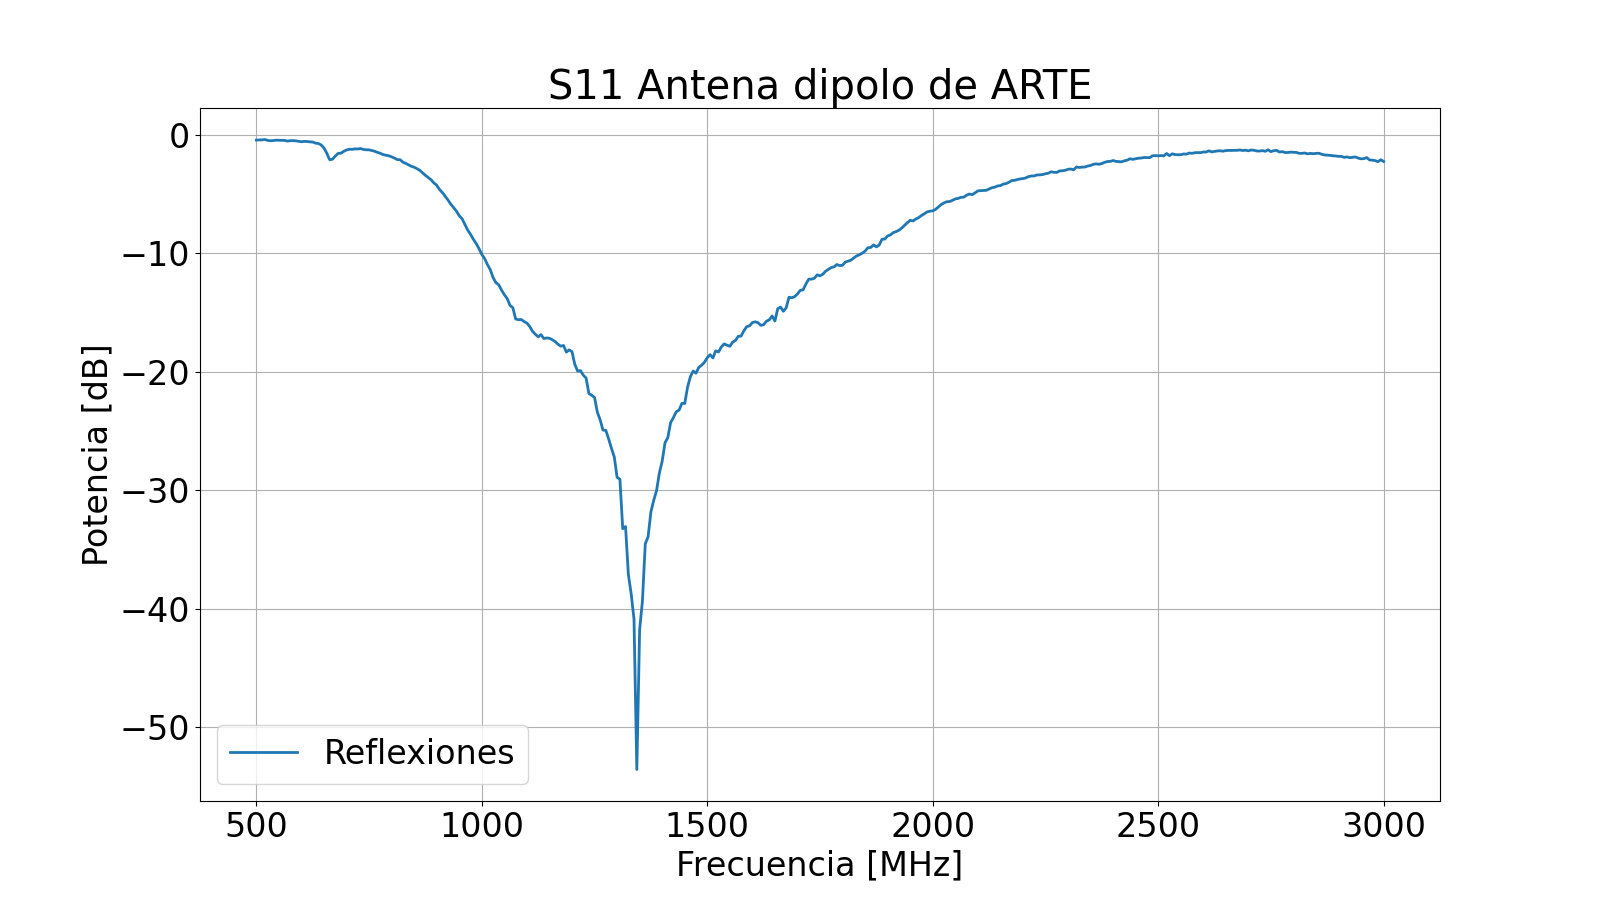
\includegraphics[width = 0.8\textwidth]{img/s11Arte}
    \caption{Ancho de banda de reflexión de una antena.}
    \label{fig:bandwidth}
\end{figure}

La figura \ref{fig:bandwidth} muestra el ancho de banda de reflexión de una antena.\\

\paragraph{Ancho de banda $S_{21}$} El ancho de banda de transmisión se define como el rango de frecuencia en el cual el parámetro de transmisión $S_{21}$ es mayor a un valor específico, comúnmente lo más cercano a 0 posible, sin embargo, cuando se utilizan componentes activos como cadenas de amplificación, este valor suele aumentar de 0 dB, lo que significa realizar un estudio más profundo del valor esperado.\\

\begin{figure}
    \centering
    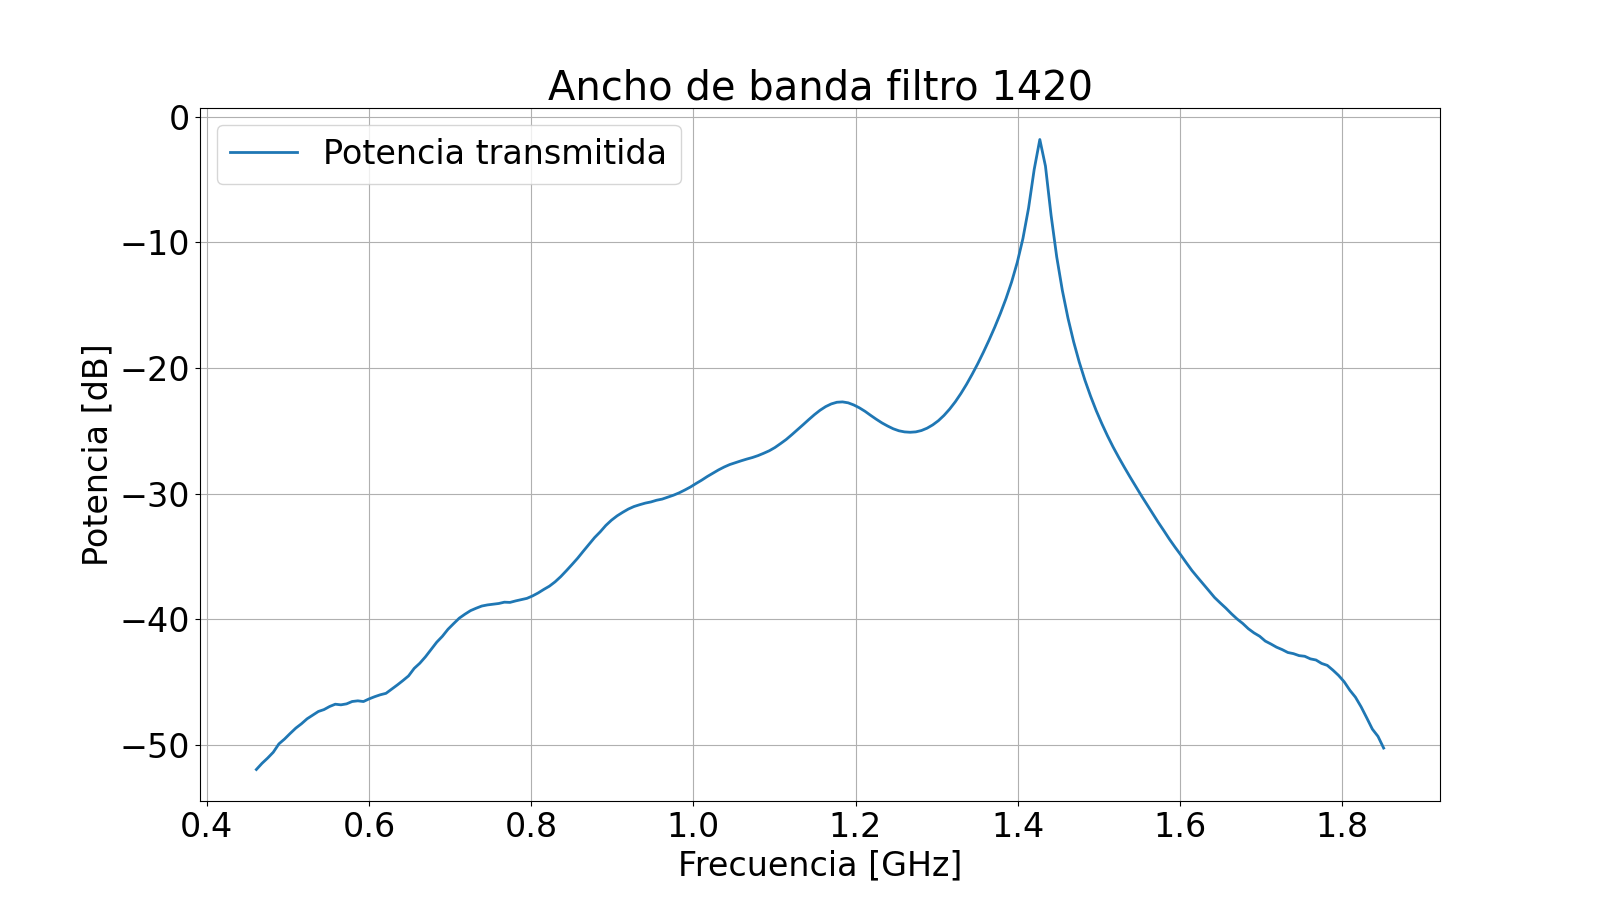
\includegraphics[width = 0.8\textwidth]{img/s21Fh1}
    \caption{Figura de una cadena de recepción con un filtro de paso de banda.}
    \label{fig:bandwidth2}
\end{figure}

La figura \ref{fig:bandwidth2} muestra el ancho de banda de un filtro de pasabanda definiendo la figura de una cadena de recepción o transmisión.\\


\subsection{Pérdidas y eficiencia}

En la propagación de ondas electromagnéticas se producen pérdidas de varias fuentes, las relacionas con el medio de propagación son las pérdidas de espacio libre y las pérdidas ohmnicas, pero en el contexto de una antena de apertura de reflector parabólico, se encuentran también las pérdidas de superficie y las pérdidas de alimentación.\\

\paragraph{Impedancia de entrada}

Los sistemas de radiofrecuencia se caracterizan por tener una impedancia asociada a la entrada y salida de los componentes que forman un sistema. Propiamente la impedancia no significa una pérdida en sí misma, pero si existen diferencias de acoplamiento de impedancia pueden empezar a encontrar pérdidas asociadas.\\

Como práctica común, se busca que la impedancia tanto de salida como entrada de los elementos de un sistema de RF sea de 50$\Omega$, pero también existen otros estándares de impedancia como los utilizados en sistemas de televisión e internet, los cuales están estandarizados a 75$\Omega$.\\

No todas las antenas una vez construidas tienen una impedancia intrínseca de 50$\Omega$, por lo que se deben utilizar elementos de adaptación de impedancia para lograr la mejor transferencia de potencia, a estos elementos se les conoce como \textit{baluns}.\\

\paragraph{Pérdidas de espacio libre}

Las pérdidas de espacio libre son las pérdidas asociadas a la propagación de ondas electromagnéticas en el espacio. Estas pérdidas son directamente proporcionales a la distancia de propagación y a la frecuencia de la señal.\\

\begin{equation}
    L_{fs} = 20log\left(\frac{4\pi d}{\lambda}\right)
\end{equation}

Donde $d$ es la distancia de propagación y $\lambda$ es la longitud de onda de la señal.\\

\paragraph{Pérdidas de superficie}

Las pérdidas de superficie están asociadas al término de eficiencia de superficie de las antenas de apertura. Estas pérdidas se deben a las imperfecciones en la superficie en relación con la longitud de onda de la señal. Se puede entender que para una longitud de onda muy grande (entre 70 cm y 10 cm) si la superficie presenta imperfecciones menores a 1 cm se puede hablar de una superficie perfecta.\\

Lo anterior da la posibilidad de utilizar superficies agujereadas o con perforaciones para reducir el peso de la antena y mejorar la eficiencia de la superficie por imperfección de curvatura.\\

\paragraph{Pérdidas ohmnicas}

Las pérdidas ohmnicas son las pérdidas asociadas a la resistencia de los materiales conductores de la antena. Estas pérdidas son directamente proporcionales a la corriente que circula por el conductor y al cuadrado de la resistencia del conductor.\\

\begin{equation}
    P_{ohm} = I^{2}R
\end{equation}

Donde $P_{ohm}$ es la potencia disipada por pérdidas ohmnicas, $I$ es la corriente que circula por el conductor y $R$ es la resistencia del conductor.\\

Estos efectos se aprecian al utilizar conductores coaxiales de grandes longitudes, un factor a considerar en la construcción de antenas.\\

\subsection{Ecuación de Friis}

La ecuación de Friis es una fórmula de transmisión para un circuito de radiofrecuencia compuesto por dos antenas, una antena transmisora u otra receptora en espacio libre \cite{Friis1946}. La ecuación se define como:\\

\begin{equation}
    \frac{P_{r}}{P_{t}} = G_{t}G_{r}\left(\frac{\lambda}{4\pi d}\right)^{2}
\end{equation}

Donde $P_{r}$ es la potencia recibida, $P_{t}$ es la potencia transmitida, $G_{t}$ es la ganancia de la antena transmisora, $G_{r}$ es la ganancia de la antena receptora, $\lambda$ es la longitud de onda de la señal y $d$ es la distancia de propagación.\\

\section{Antenas parabólicas}

Una antena parabólica es una antena de apertura que se compone de una superficie reflectante parabólica y una antena alimentadora. Se caracterizan por tener una alta directividad y ganancia, por lo que son utilizadas en aplicaciones de comunicación de largo alcance y en radiotelescopios, donde se requiere una alta sensibilidad.\\


\subsection{Tipos de antenas parabólicas}

Las antenas parabólicas se pueden clasificar en 4 tipos de configuraciones, \textit{Cassegrain}, \textit{Gregorian}, \textit{off-axis} o fuera de foco y \textit{axial feed} o Foco Primario.\\

\paragraph{Cassegrain}

Las antenas de tipo Cassegrain, son aquellas que utilizan un reflector secundario para redirigir la radiación hacia la antena alimentadora. El reflector secundario es un hiperboloide de revolución que se ubica en el foco de la parábola principal y se orienta hacia la antena alimentadora.

\begin{figure}
    \centering
    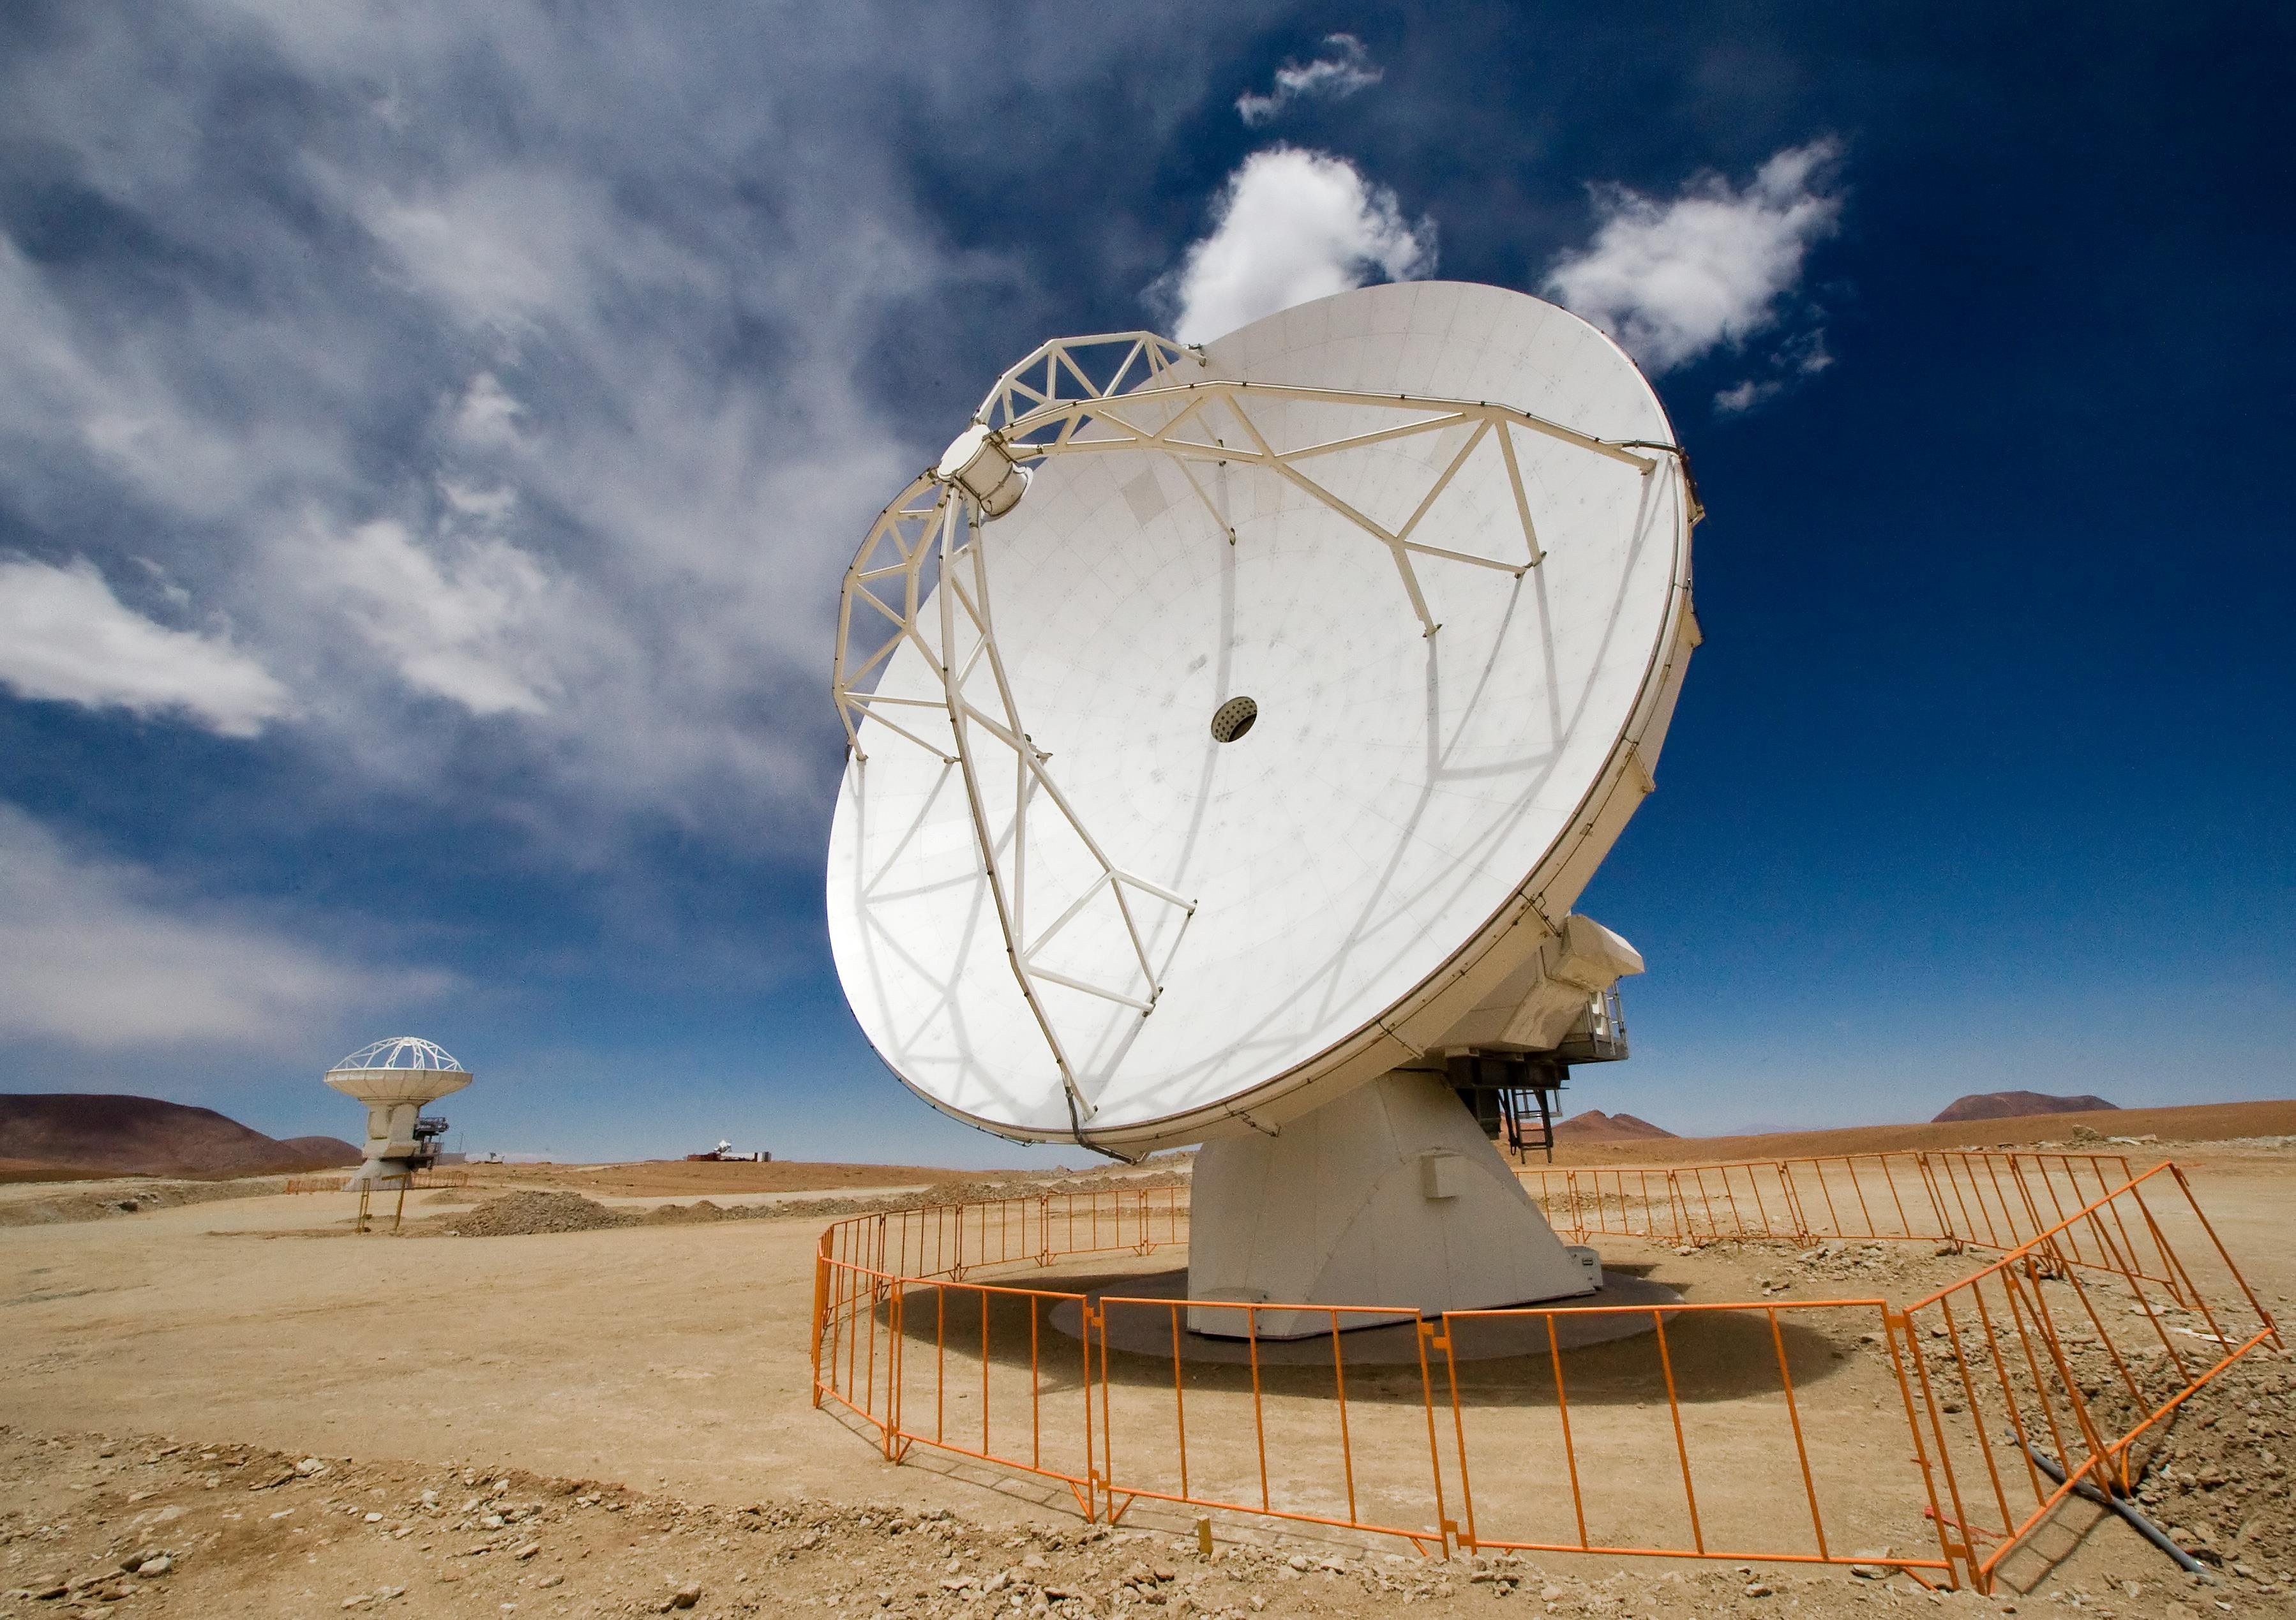
\includegraphics[width = 0.8\textwidth]{img/cassegrain.jpg}
    \caption{Antena de 12 metros Vertex tipo Cassegrain en el observatorio de ALMA.}
    \label{fig:cass}
\end{figure}

\paragraph{Gregorian}

Las antenas de tipo Gregorian, son aquellas que utilizan un reflector secundario para redirigir la radiación hacia la antena alimentadora. El reflector secundario es un elipsoide de revolución que se ubica en el foco de la parábola principal y se orienta hacia la antena alimentadora.

\begin{figure}
    \centering
    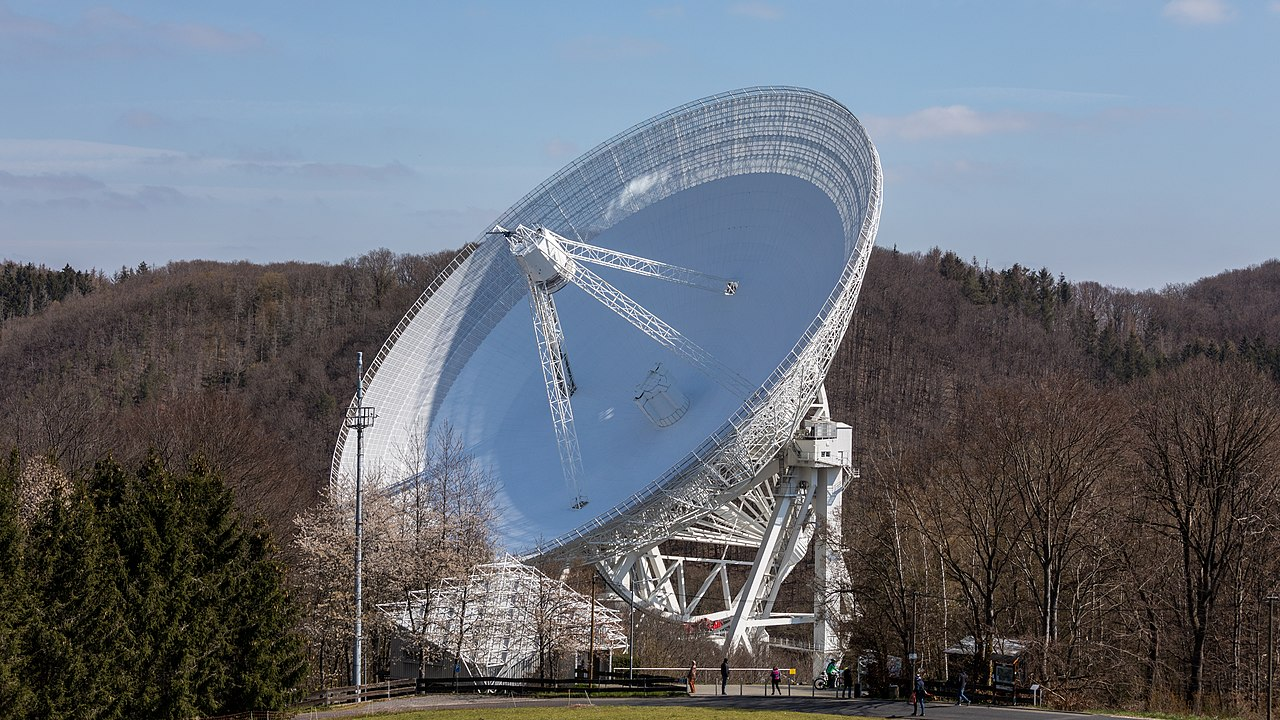
\includegraphics[width = 0.8\textwidth]{img/gregorian.jpg}
    \caption{Telescopio Effelsberg de 100 metros de tipo Gregorian.}
    \label{fig:greg}
\end{figure}

\paragraph{Off-axis}

Las antenas de tipo \textit{off-axis} o fuera de foco, son aquellas en las cuales la antena alimentadora se encuentra fuera de los ejes de la parábola principal, extendiendo el reflector principal. Este tipo de antenas se utilizan en aplicaciones donde se requiere una mayor área de cobertura revisando la obstrucción de la antena alimentadora.

\begin{figure}
    \centering
    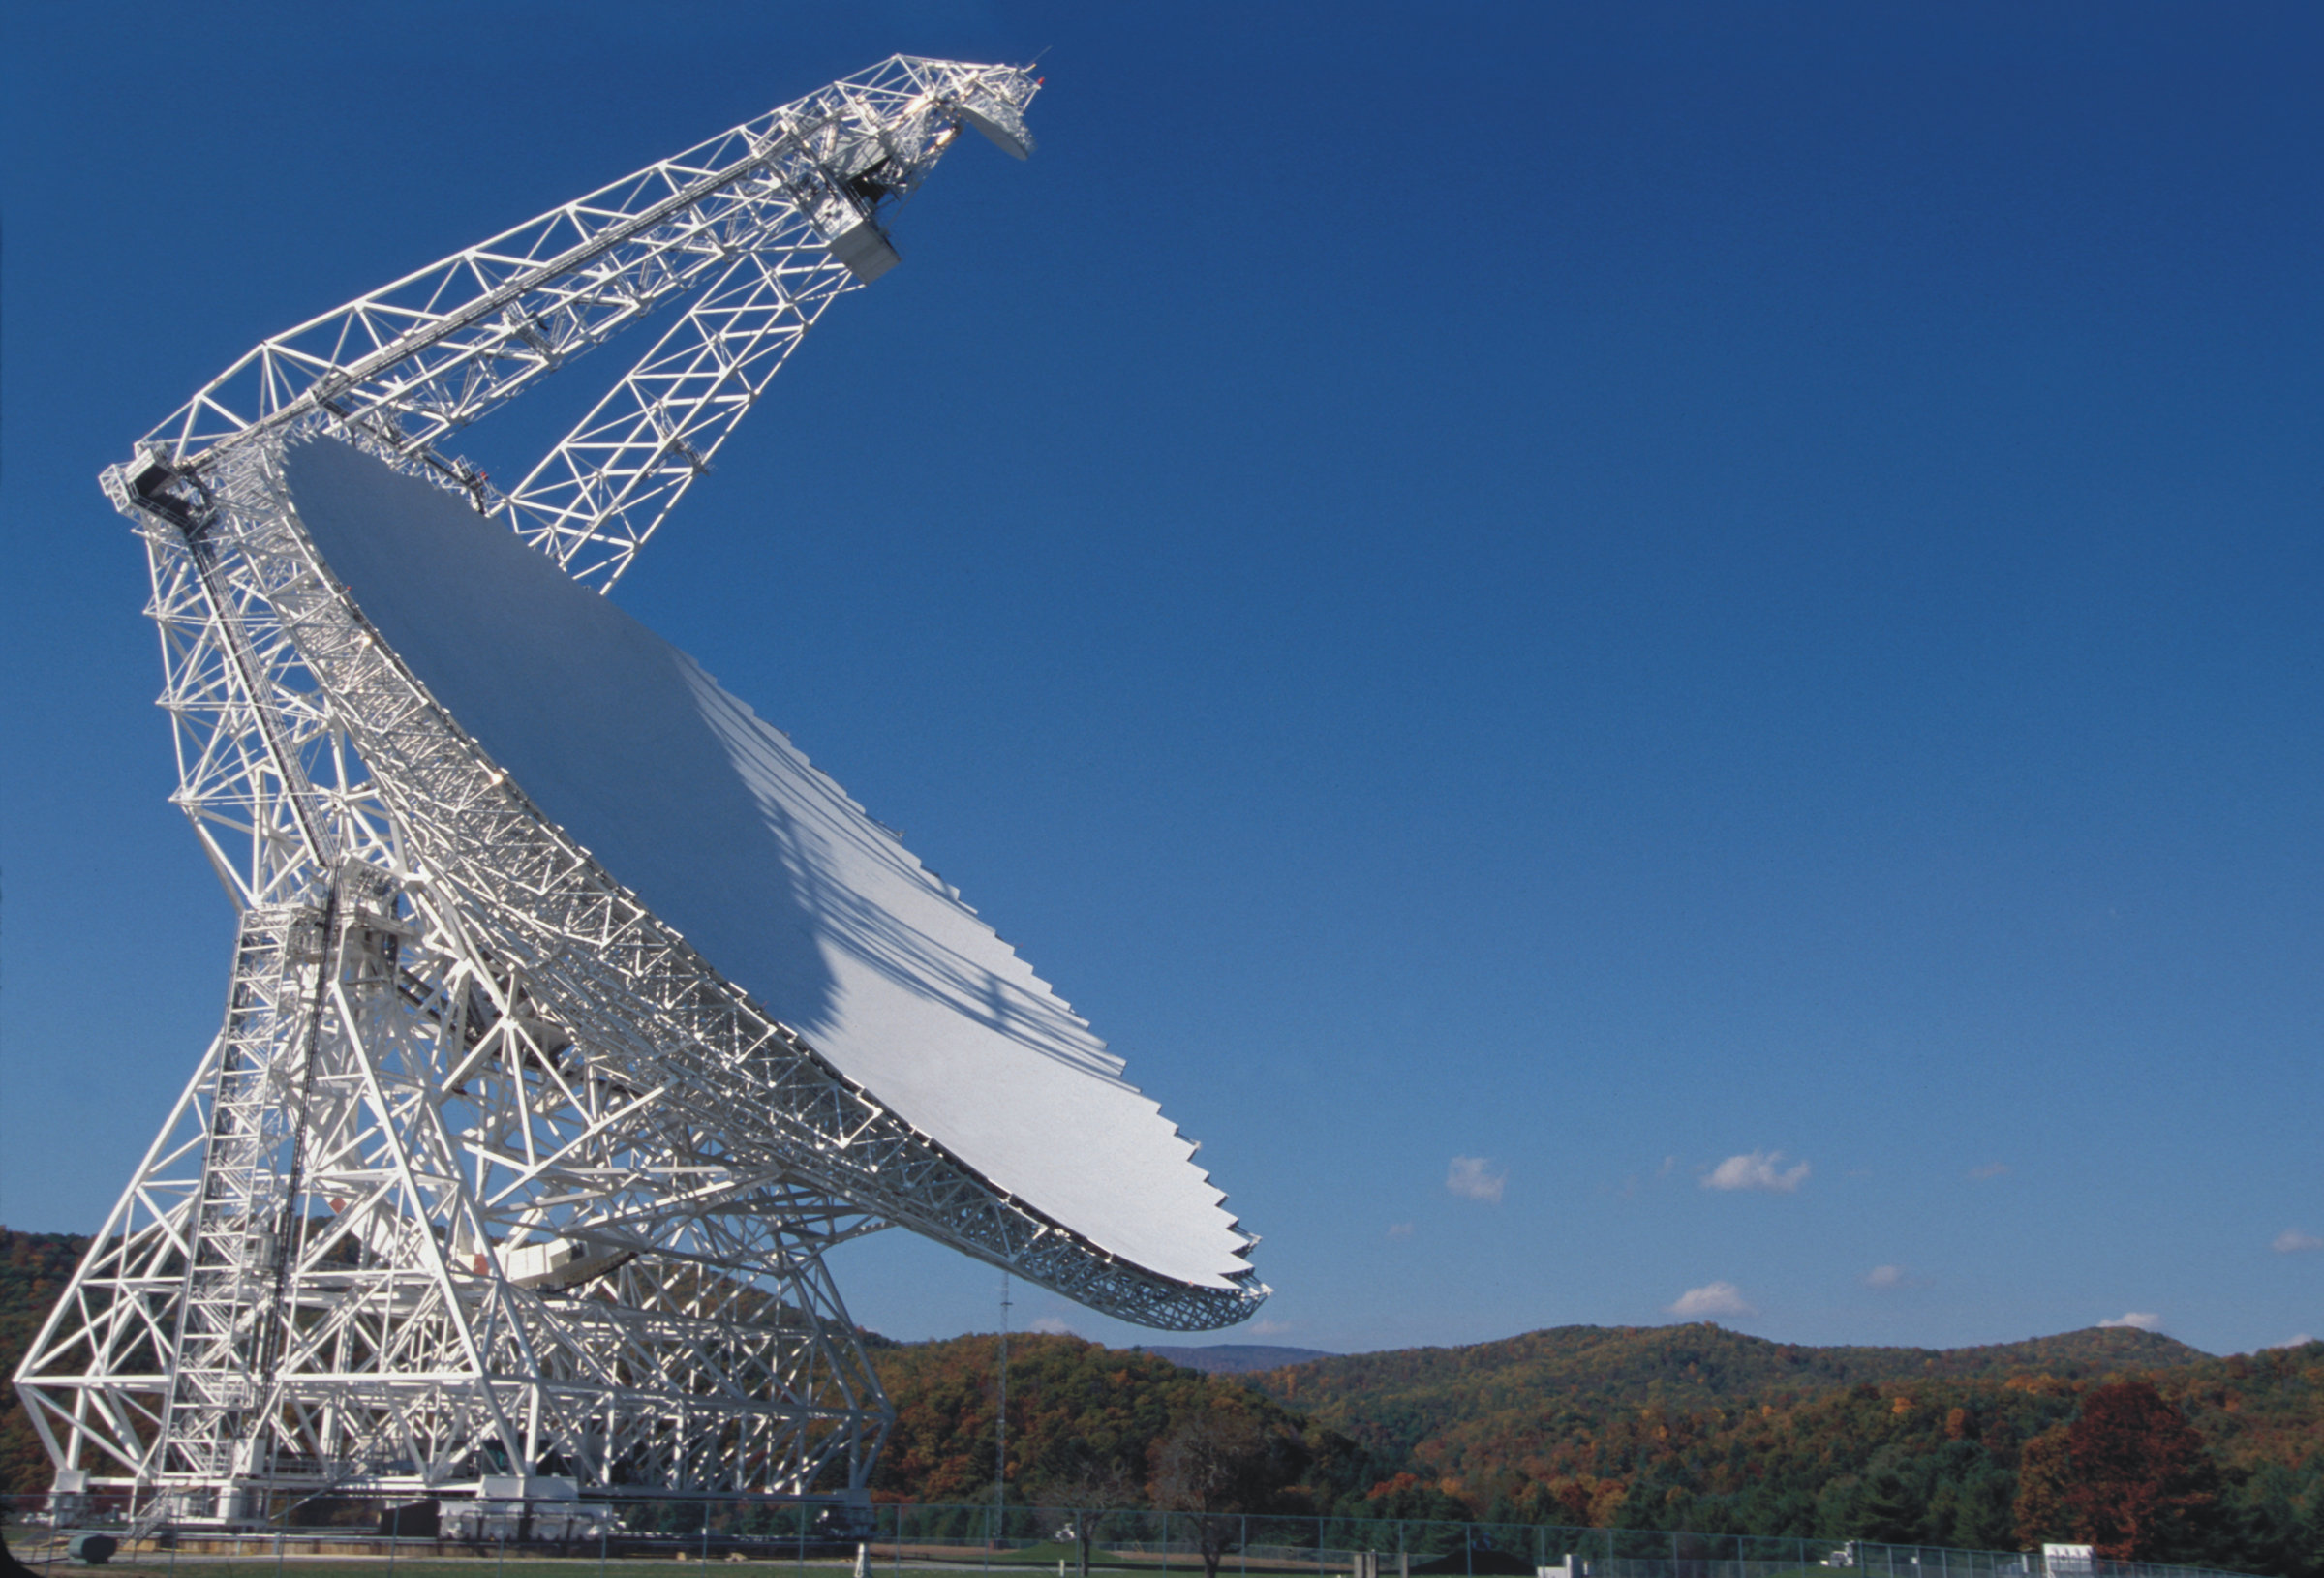
\includegraphics[width = 0.8\textwidth]{img/off-axis.jpg}
    \caption{Telescopio GBT (Green Bank Telescope) de 100 metros de tipo \textit{off-axis}.}
    \label{fig:off}
\end{figure}


\paragraph{Foco primario}

Las antenas de tipo foco primario, son aquellas donde la antena alimentadora se encuentra en el foco de la parábola principal. Este tipo de antenas son más simples de construir, pero tienen otros desafíos ópticos y de diseño.\\

\subsection{Antenas de alimentación}

Las antenas alimentadoras son los elementos ubicados en el foco de la parábola principal que capturan la radiación concentrada por el reflector. Estas antenas deben tener un patrón de radiación adecuado para el tipo de diseño de la antena parabólica.\\

Las antenas alimentadoras pueden ser de distintos tipos, como antenas de parche, antenas de bocina, antenas yagui-uda, antenas log-periódicas, antenas de semiespacio, entre otras. El tipo de antena alimentadora a utilizar dependerá del tipo de antena parabólica y de la aplicación de la antena, sin embargo, las antenas de bocina son las más utilizadas en antenas parabólicas de reflector secundario.\\


\section{Receptores heterodinos}

Los receptores comúnmente utilizados en radioastronomía son bastante similares a los utilizados en telecomunicaciones. La característica principal de estos receptores es convertir las señales incidentes a un rango de frecuencia menor conservando la fase y la amplitud, esta frecuencia se le conoce como frecuencia intermedia o IF, la cual es procesada a posteriori para extraer su información \cite{Finger2013}.\\

En todos los receptores heterodinos se utiliza un mezclador para realizar la conversión de frecuencia, este es un dispositivo no lineal que procesa las señales con una señal de referencia conocida como oscilador local.\\


\subsection{Radio definida por software}

Una radio definida por software o SDR, es un receptor heterodino con un oscilador reprogramable y entrega la señal de IF a un computador para su procesamiento. Estos receptores se pueden reconfigurar para sintonizar distintas frecuencias, para luego entregar las muestras digitales a un computador y así procesar la señal, como por ejemplo, realizar una transformada de Fourier para obtener el espectro de la señal.\\

%\subsection{Transformada Rápida de Fourier}




\section{Radiotelescopios}

Tal como los telescopios ópticos que concentran la luz visible en un foco, la amplifican y procesan para que sea analizada por diversos instrumentos, también los radiotelescopios concentran la luz de las ondas de radio de las estrellas y otros cuerpos celestes. Estos telescopios son diseñados para observar las ondas más grandes de la luz, desde 1 mm a 10 metros de longitud de onda. \cite{nraoRadioTelescopes}\\

Un radiotelescopio a diferencia de un telescopio óptico posee una ventaja única. La radiación observada es coherente, por lo que existen los amplificadores coherentes, los cuales mantienen la información de la fase de la señal. Esta cualidad permite la construcción de interferómetros y telescopios de apertura sintética \cite{Ransom2016}.\\ 

\subsection{Línea de Hidrógeno Neutro}

El movimiento de un electrón en un átomo de Hidrógeno neutro genera un campo magnético que se acopla con los espines del protón y el electrón. \quotes{Este acople da cuenta de la radiación a 1420 MHz que viene de la transición entre dos niveles energéticos de primer nivel del estado fundamental del Hidrógeno} \cite{Restrepo2023}.\\

La línea de hidrógeno neutro o H1, es una de las líneas espectrales más importantes en radioastronomía, ya que permite observar la distribución de gas en las galaxias y la evolución del universo primitivo. También es una de las más estudiadas y catalogadas por muchos otros telescopios.\\

\subsection{CHARTS y FRB}

Los fenómenos astrofísicos transitorios de radio o FRB, son eventos de extremadamente corta duración y origen desconocido que ocurren en un amplio rango de frecuencias. Estos pulsos inspiraron el proyecto CHARTS, para apoyar su búsqueda y estudio.\\

El proyecto CHARTS, es una colaboración entre la Universidad de Chile y la Universidad de Toronto con el objetivo de construir un arreglo de 128 sintonizadas para operar en el rango de 300 MHz a 500 MHz en el marco de la búsqueda de FRB.\\


\section{Telescopio CPT}

El telescopio CPT, \textit{CHARTS Pathfinder Telescope}, es un telescopio de 3 metros de diámetro con una configuración de foco primario. Este telescopio se encuentra en la cumbre del cerro Calán en Santiago de Chile, siendo parte del departamento de astronomía de la Facultad de Ciencias Físicas y Matemáticas de la Universidad de Chile.\\

El reflector de este telescopio es un paraboloide de 3 metros de diámetro, con una estructura de aluminio unida con remaches y pernos. Su superficie reflectante es de malla de acero galvanizado con separación de 6 mm, el anillo exterior es de una cinta de aluminio de 3x20 mm. El soporte del alimentador es de 4 perfiles de aluminio de 2x2 cm de 2 metros de largo \cite{rfhamdesign3meterdish}.\\

La eficiencia de superficie que estima el fabricante es de 65\% teniendo su ganancia máxima a 5760 MHz con 43.3 dB y a 1296 MHz con 30.3 dB. Tanto el reflector como la montura alt-azimutal son de la compañía holandesa \textit{RFHamdesign}.\\

\begin{figure}
    \centering
    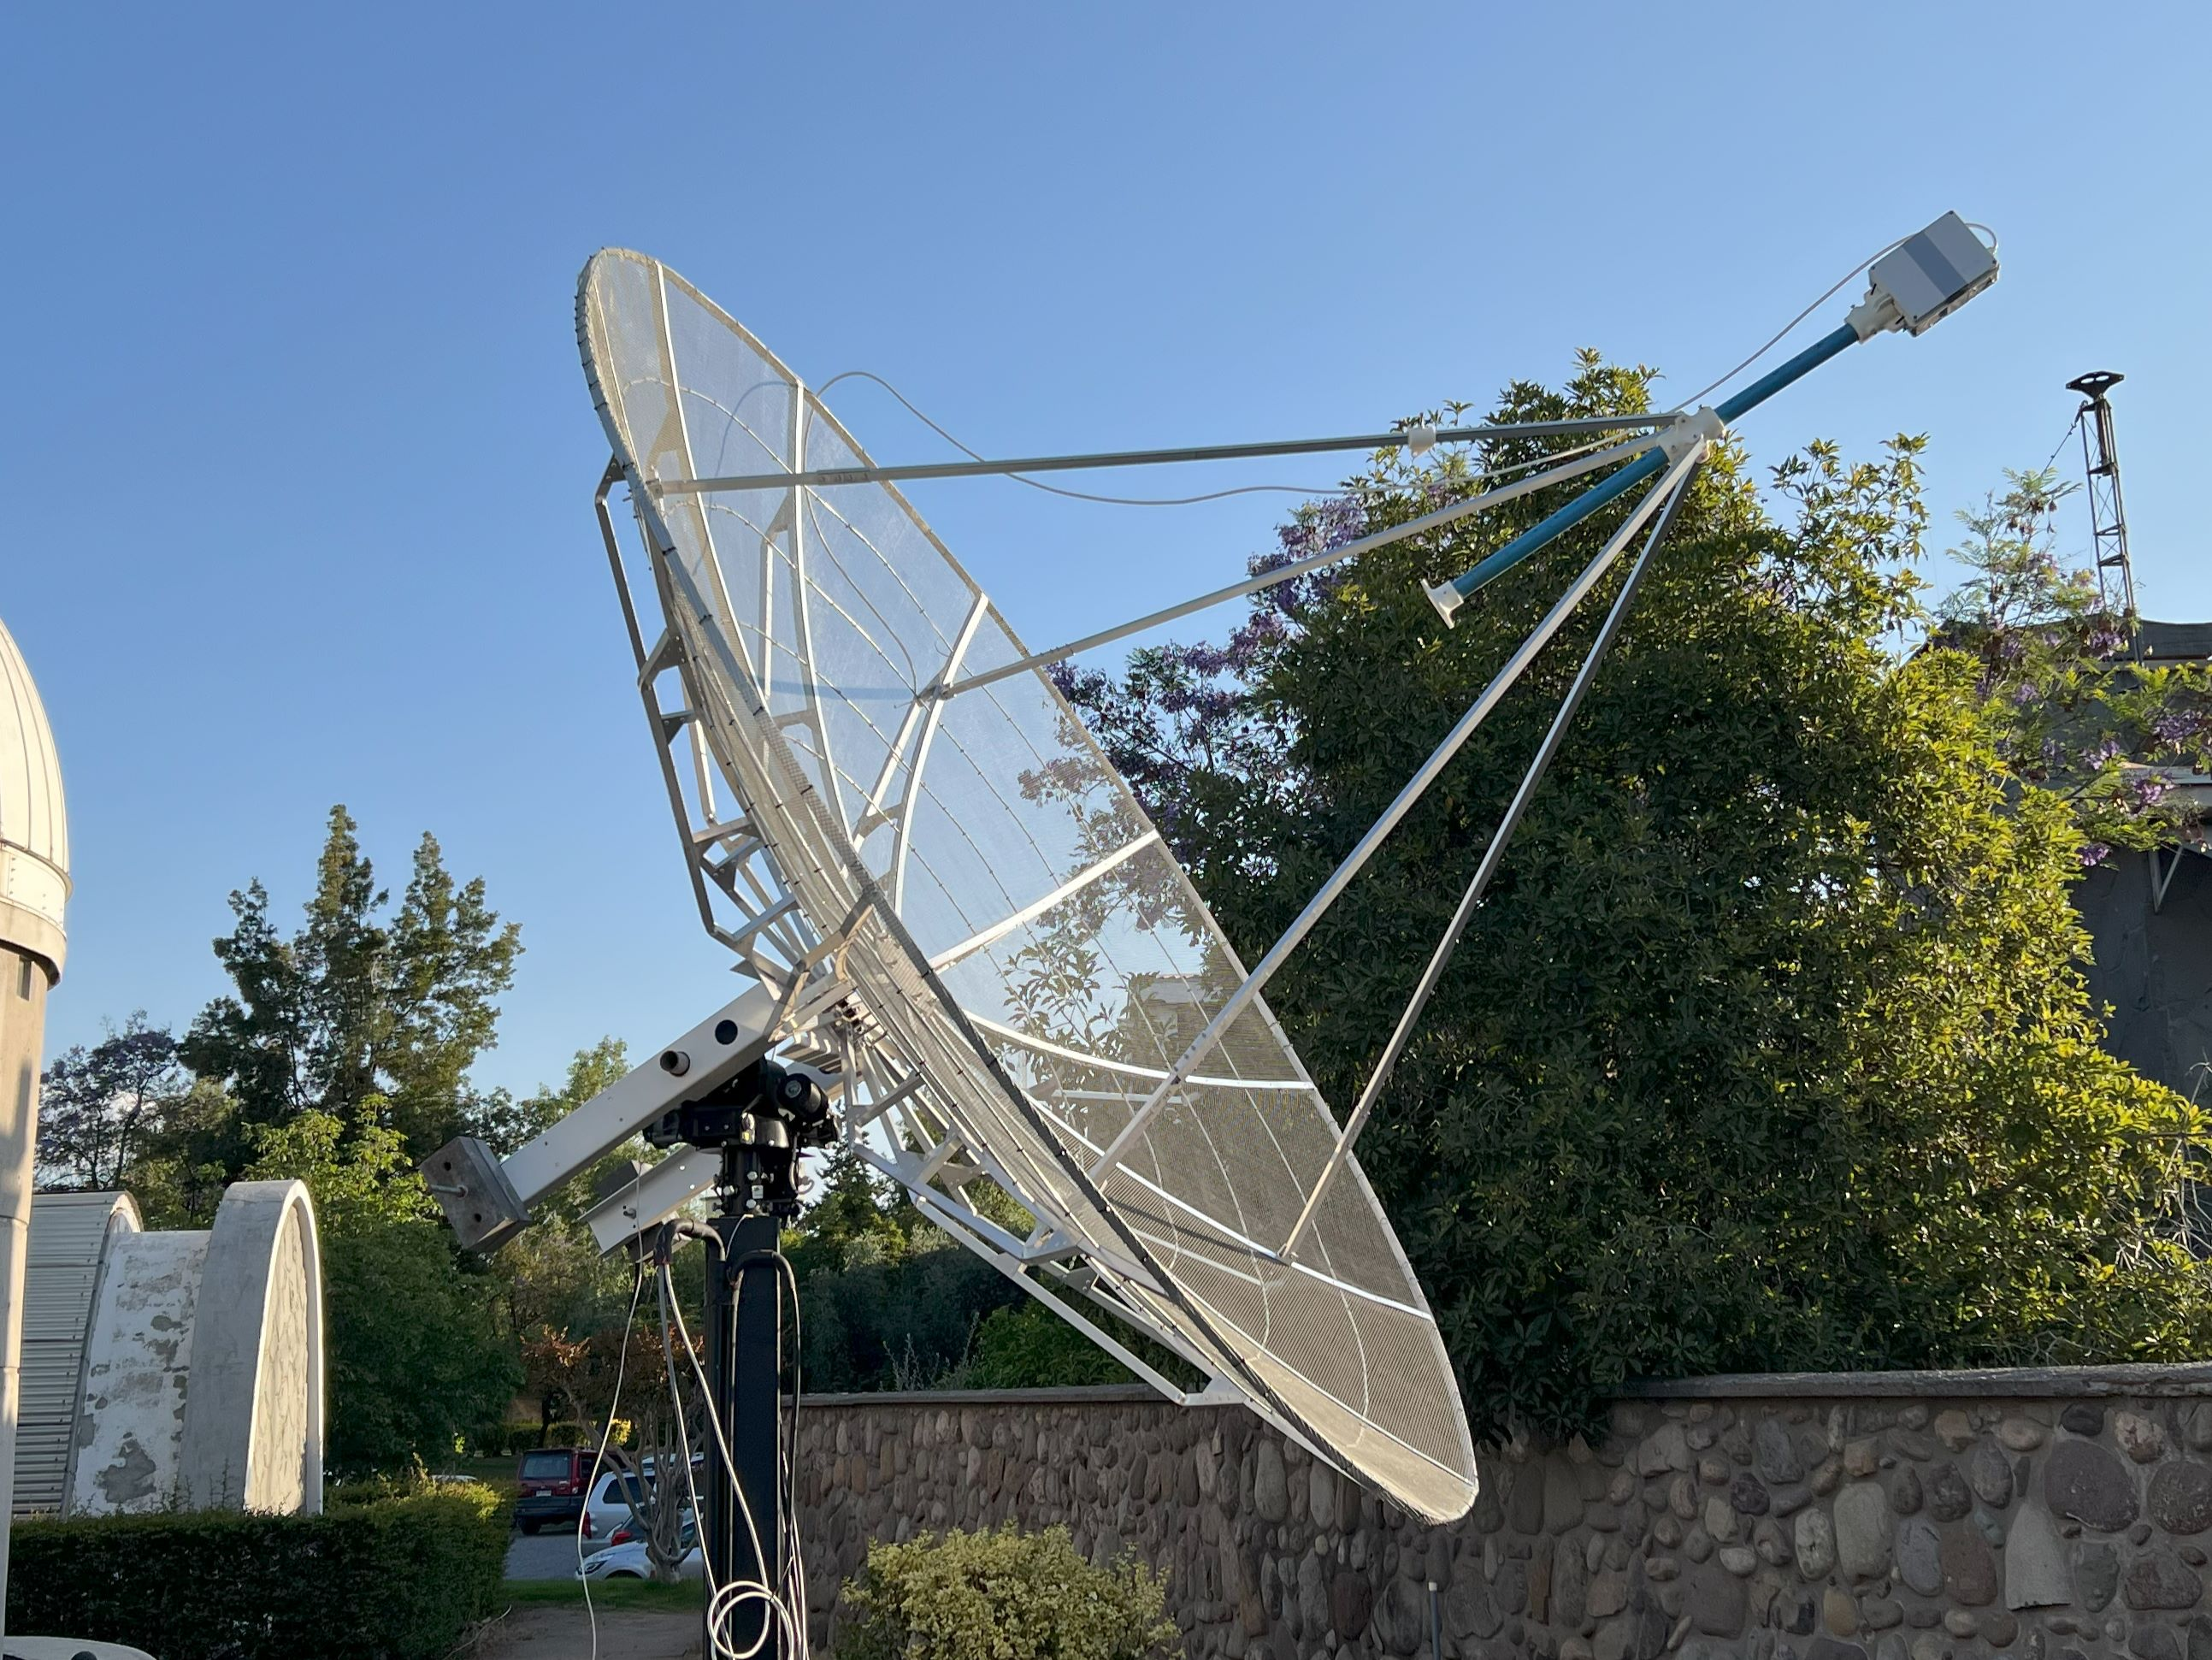
\includegraphics[width = 0.8\textwidth]{img/cpt_tracking}
    \caption{Telescopio CPT en el cerro Calán siguiendo el centro de la galaxia.}
    \label{fig:cpt}
\end{figure}

El propósito para poner en servicio este telescopio es observar la línea espectral de hidrógeno neutro de 21 cm de longitud de onda, para caracterizar todos los aspectos de la antena y comenzar a realizar observaciones de radioastronomía. Luego se ampliarán sus capacidades para apoyar al proyecto CHARTS en la banda de 300 MHz a 500 MHz y hacer observaciones solares de alto ancho de banda desde 1 GHz a 6 GHz.\\

\section{Métodos de caracterización}

Los siguientes métodos son los más comunes en la caracterización de antenas y radiotelescopios para medir su desempeño y definir sus capacidades como instrumentos astronómicos.\\

\subsection{Medición de patrón de radiación}

El método más directo para la medición del patrón de radiación es el de campo lejano y al tratarse de antenas de apertura de grandes dimensiones, presenta varios desafíos prácticos y técnicos, especialmente a altas frecuencias \cite{Astudillo2014}.\\

\begin{figure}
    \centering
    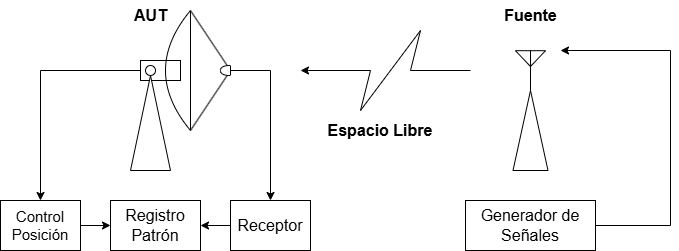
\includegraphics[width = 0.8\textwidth]{img/farfielddiag}
    \caption{Diagrama de un sistema de medición de patrón de radiación para una antena bajo prueba (AUT) en campo lejano.}
    \label{fig:farfield}
\end{figure}

La figura \ref{fig:farfield} muestra un diagrama de un sistema básico necesario para poder realizar la medición, el cual requiere la antena objetivo, la que se quiere caracterizar. La antena fuente, que es la que generara la radiación para medir la antena objetivo. Además de todo el equipo e instrumentación necesaria.\\

\subsection{Medición de la temperatura de ruido}

Para medir la temperatura de ruido de un sistema, se puede utilizar el método de factor Y, el cual consiste en utilizar una fuente de ruido de ENR, conocida como \textit{Excess Noise Ratio} o la relación de exceso de ruido, la cual se conecta a la antena y se mide la potencia de ruido en la salida del receptor.\\

La medición se realiza obteniendo la temperatura del sistema cuando se enciende la fuente de ruido y cuando se apaga, siendo estas temperaturas como $T_{hot}$ y $T_{cold}$ o temperatura caliente y temperatura fría respectivamente.\\

El ruido de ENR se obtiene a 2 \quotes{temperaturas de ruido} conocidas, una a temperatura ambiente y otra a la temperatura con la fuente encendida.\\

\begin{equation}
    ENR = \frac{T_{hot} - 290}{290}
\end{equation}

Considerando la temperatura ambiente como 290 grados K. ENR se logra polarizando la fuente de ruido y para obtener el factor Y utilizamos la siguiente ecuación:\\

\begin{equation}
    Y = \frac{\frac{T_{hot}}{T_{cold}} + \frac{T_{noise}}{T_{cold}}}{1 + \frac{T_{noise}}{T_{cold}}}
\end{equation}

Donde $T_{noise}$ es la temperatura de ruido del sistema. Así para obtener la figura de ruido se necesita el factor de ruido F, $F=T_{noise}/T_{cold} +1 $, para luego reemplazarlo en $NF = 10log(F)$\cite{analogNoiseFigure}.\\


%\section{Estado del arte}





% \section{Conceptos previos}
% \subsection{Radiotelescopio}

% En la astronomía clásica, se utilizan telescopios que operan en el rango visible del espectro electromagnético, el mismo rango que tiene el ojo humano, donde estos actúan como el receptor o, al mismo tiempo, una cámara fotográfica. En contraste, un radiotelescopio es un instrumento que observa en longitudes de onda mucho más grandes en el espectro de radio. Estos telescopios, usualmente, son constituidos por un reflector parabólico que concentra la luz obtenida en su foco, donde se ubica un receptor de radio.\\

% Un telescopio de radio tiene consideraciones distintas a uno óptico, ya que el anterior puede observar con múltiples receptores a la vez como lo es el caso de una cámara fotográfica, pero uno de radio, debe tener un receptor de mayor envergadura proporcional con el tamaño de la longitud de onda, lo que limita el número de receptores a uno en la gran mayoría de los casos.\\

% Otro punto importante a destacar, es la característica de ciencia que se puede realizar con estos telescopios, ya que para el caso de la línea de Hidrógeno, se pueden observar fuentes que no necesariamente provienen de estrellas o, para frecuencias más bajas, estrellas con que irradian fuera del rango visible.

% \subsection{Línea de Hidrógeno Neutro}

% El movimiento de un electrón en un átomo de Hidrógeno neutro, genera un campo magnético que se acopla con los espines del protón y el electrón. \quotes{Este acople da cuenta de la radiación a 1420 MHz que viene de la transición entre dos niveles energéticos de primer nivel del estado fundamental del hidrógeno} \cite{Restrepo2023}.\\

% Observar H1 permite estudiar la evolución del universo primitivo, rescatando información proveniente de la transición de la \quotes{Época Oscura} a la formación de las primeras fuentes de luminosas del universo.

% \subsection{CHARTS y FRB}

% Los fenómenos astrofísicos transitorios de radio o FRB, son eventos de extremadamente corta duración y origen desconocido que ocurren en un amplio rango de frecuencias. Estos pulsos inspiraron el proyecto CHARTS, para apoyar su búsqueda y estudio.\\

% El proyecto CHARTS, es una colaboración entre la Universidad de Chile y la Universidad de Toronto con el objetivo de construir un arreglo de 128 sintonizadas para operar en el rango de 300MHz a 500MHz en el marco de la búsqueda de FRB.

% \subsection{Polarización}

% La polarización de una antena hace referencia a la polarización del campo eléctrico y magnético que produce al irradiar potencia al medio. Convencionalmente, se utilizan 2 polarizaciones para las observaciones astronómicas y para las telecomunicaciones, la polarización lineal y la polarización circular.\\

% \begin{figure}
% \centering
% 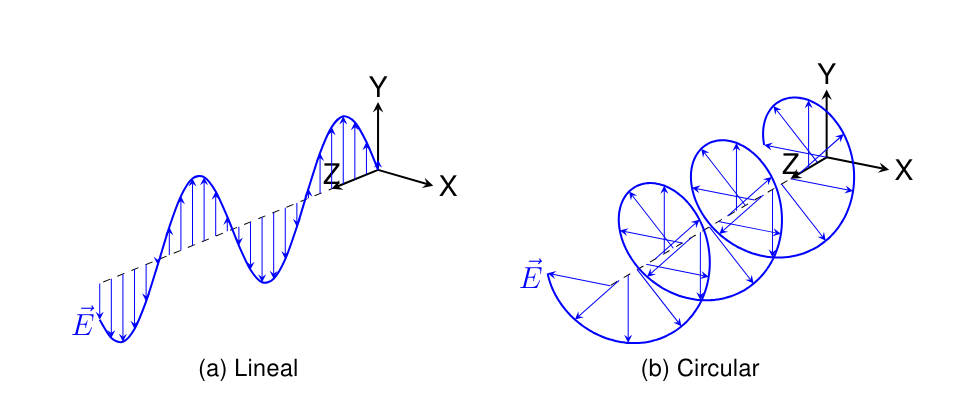
\includegraphics[width = 15cm]{img/pol.png}
% \caption{A la izquierda se tiene una polarización lineal del campo electromagnético y a la derecha una polarización circular izquierda\cite{Astudillo2014}.}
% \label{fig:pol}
% \end{figure}

% La polarización linear, se genera con el campo eléctrico contenido en un plano, como se puede ver en la figura \ref{fig:pol}. En contraste, la polarización circular se produce en un caso particular cuando el campo eléctrico rota con una frecuencia constante en torno a un eje y su magnitud es constante. De lo contrario, se produce una polarización elíptica en torno al eje de propagación, tal como se observa en la figura anterior.\\

% Las distintas polarizaciones, se pueden generar por medios constructivos en la geometría de la antena o medios de alteración de fase, ya sea por efectos de largo eléctrico o modulaciones electrónicas para generar el desfase de las líneas alimentadoras.

% \subsection{Antenas de Apertura}

% Las antenas de apertura son aquellas que su funcionamiento es caracterizado por el campo generado en una superficie reflectante, la cual se denomina como apertura. Dentro de las antenas de apertura están las antenas de apertura parabólica que utilizan una superficie parabólica para irradiar potencia. Existen 4 tipos de configuraciones para las antenas parabólicas, \textit{Cassegrain}, \textit{Gregorian}, \textit{off-axis} o fuera de foco y \textit{axial feed} o Foco Primario. Esta última es el que se utilizará para el proyecto.\\

% Estas antenas concentran la radiación en un punto focal dependiendo de su geometría de paraboloide. Usualmente, se instala la antena alimentadora en el foco de la parábola o en el foco de la segunda parábola para las antenas \textit{Cassegrain} y \textit{Gregorian}.\\

% \begin{figure}
% \centering
% 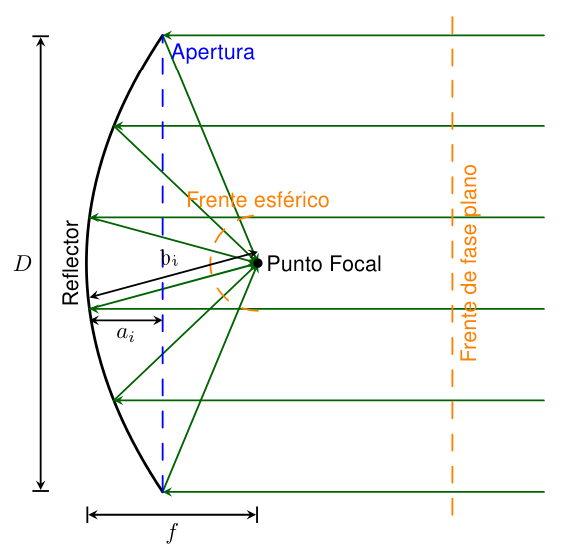
\includegraphics[width = 10cm]{img/parabola.png}
% \caption{Geometría característica de un reflector parabólico para el tipo de Foco Primario\cite{Astudillo2014}.}
% \label{fig:parabola}
% \end{figure}

% La representación de seguimiento de rayos en dos dimensiones para un reflector parabólico en la figura \ref{fig:parabola}, hace referencia al tipo de configuración a utilizar en la construcción del reflector del nuevo radio telescopio.


% \subsection{Antena Alimentadora}

% La antena alimentadora, es aquella antena que captura la radiación proveniente de los reflectores. Se debe ocupar una antena con un patrón de radiación directivo, con el objetivo de captar la mayor cantidad de la luz concentrada por el reflector.\\

% Ejemplos de antenas directivas:

% \begin{itemize}
% \item Yagi-Uda
% \item Bocina
% \item Log-Periódica
% \item Antenas de semi espacio
% \item Antenas de parche
% \end{itemize}

% \subsection{Receptor Heterodino}

% Los receptores heterodinos, o coherentes, son los más usados en la radioastronomía. Su función característica es convertir una señal de alta frecuencia a un rango de menor frecuencia, conservando la información de fase y de amplitud para poder ser digitalizada con facilidad\cite{Finger2013}. Para esto, los receptores utilizan un mezclador con un oscilador local para adquirir la señal desde la antena alimentadora para luego ser procesada digitalmente.\\

% \begin{figure}
% \centering
% 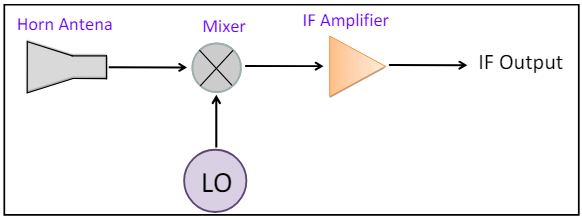
\includegraphics[width = 10cm]{img/heterodine.png}
% \caption{Diagrama de bloques de un receptor heterodino para astronomía de tipo DSB.}
% \label{fig:radio}
% \end{figure}

% La figura \ref{fig:radio} corresponde a un diagrama de bloques de la configuracion más simple para un receptor heterodino. Contiene una antena receptora, un mezclador de radio frecuencia, un oscilador local y un amplificador de bajo ruido.

% \section{Estado del Arte}

% El estado del arte para radiotelescopios, en particular de radios telescopios de reflectores con diámetros de 3 metros o menos. En este caso, la principal línea de desarrollo es en la radio-interferometría y el uso de sistemas de bajo ruido, a la vez que la disminución de los costos para nuevos instrumentos.\\

% Los esfuerzos para la búsqueda de FRB y, específicamente, en la detección del origen de estos pulsos de alta energía, puede lograrse con el uso de \textit{Pathfinding} al correlacionar 2 telescopios separados por largas distancias para hacer interferometría de línea de base muy larga, o VLBI por su sigla en inglés (T. A. Cassanelli, 2021). Experimento que se quiere hacer con el proyecto CHARTS y este nuevo telescopio.\\

% Luego, en el contexto de la construcción un nuevo radiotelescopio para observar la línea de 21cm, se tienen los siguientes exponentes que implementan diversas técnicas que inspiran el desarrollo y operación que se desea con el telescopio CPT.\\


% \subsection{Telescopio Mini}

% \begin{figure}
% \centering
% 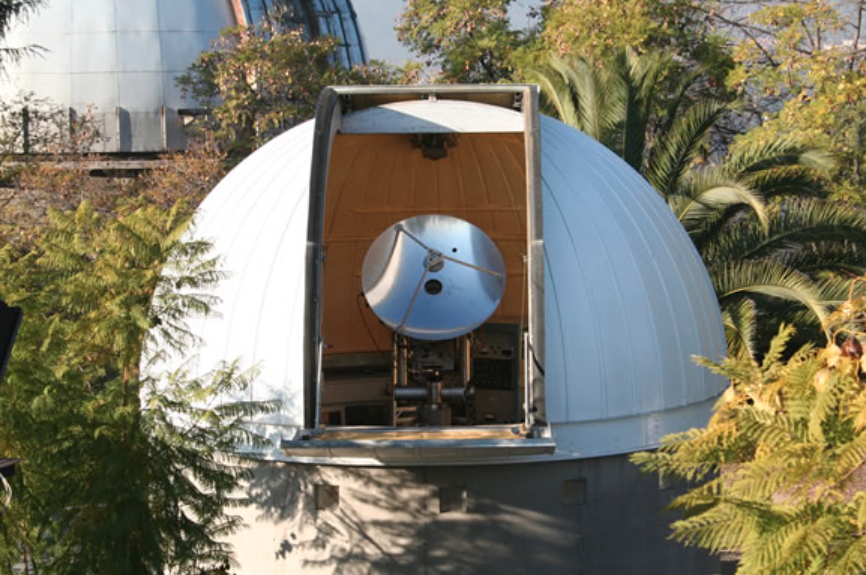
\includegraphics[width = 12cm]{img/mini.png}
% \caption{Telescopio MINI en el Observatorio Cerro Calan de la Facultad de Ciencia Físicas y Matemáticas de la Universidad de Chile\cite{DAS2024}}
% \label{fig:mini}
% \end{figure}

% El telescopio de la figura \ref{fig:mini}, se encuentra en el cerro Calán, a pocos metros de la ubicación de los cimientos para, CPT, ejemplificando las consideraciones de operar en un ambiente extremadamente saturado de interferencia de radiofrecuencia que se puede encontrar en el centro de la ciudad principal del país como Santiago.

% \subsection{Telescopio FAST}

% \begin{figure}
% \centering
% 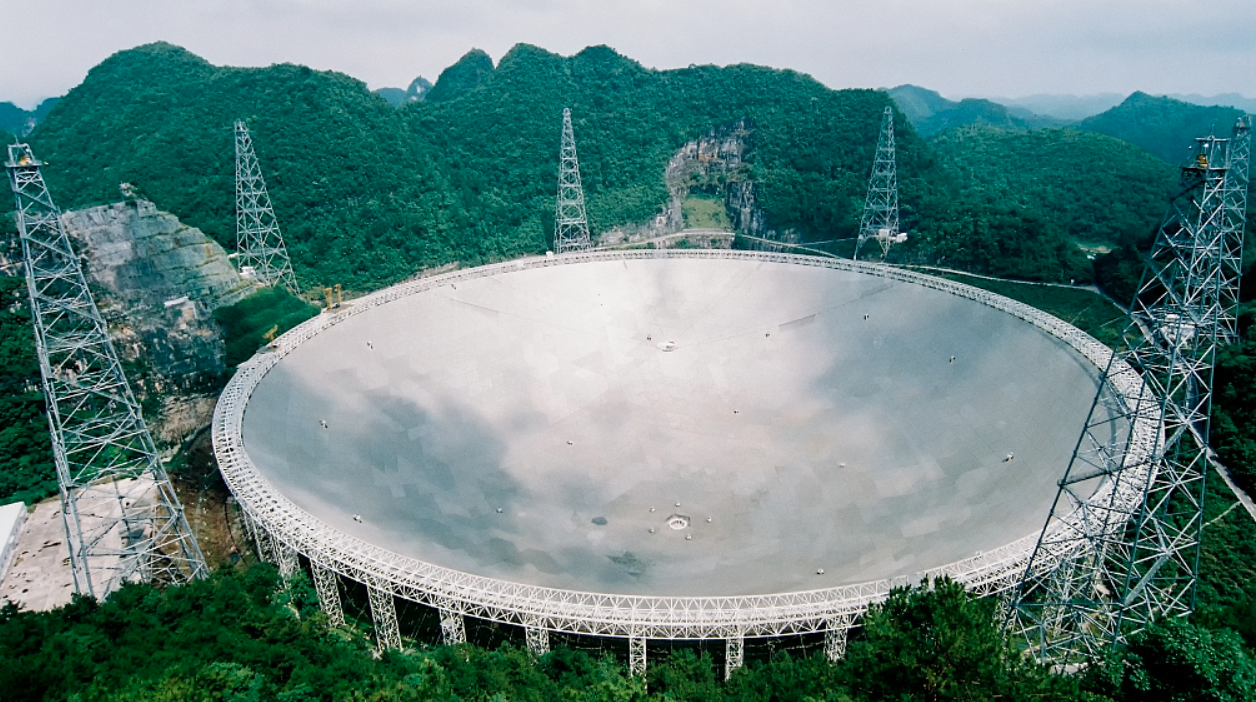
\includegraphics[width = 12cm]{img/fast.png}
% \caption{Telescopio Fast en la provincia de Guizhou, China \cite{FAST2024}.}
% \label{fig:fast}
% \end{figure}

% La figura \ref{fig:fast}, corresponde a un telescopio de 500 metros de apertura con un alimentador posicionado en el foco de la superficie parabólica primaria que puede hacer observaciones de la linea de 21cm y de FRB. El cual se ubica en China, en la provincia de Guizhou.

% \subsection{Telescopio SRT}

% \begin{figure}
% \centering
% 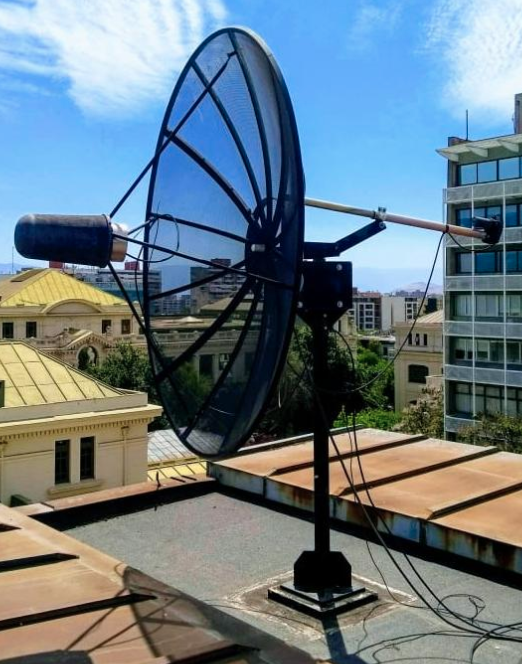
\includegraphics[width = 6cm]{img/srt.png}
% \caption{Telescopio SRT del MIT en la azotea del departamento de ingeniería eléctrica de la FCFM\cite{Curotto2019}.}
% \label{fig:srt}
% \end{figure}

% El Telescopio de la figura \ref{fig:srt}, se encuentra ubicado en la azotea del edificio del Departamento Ingeniería Eléctrica de la Universidad de Chile, equipado con receptores y filtros diseñados para observar la línea de Hidrógeno neutro. El material de sus reflectores es similar al que se utilizará en CPT.

% \subsection{Observatorio CHIME}

% \begin{figure}
% \centering
% 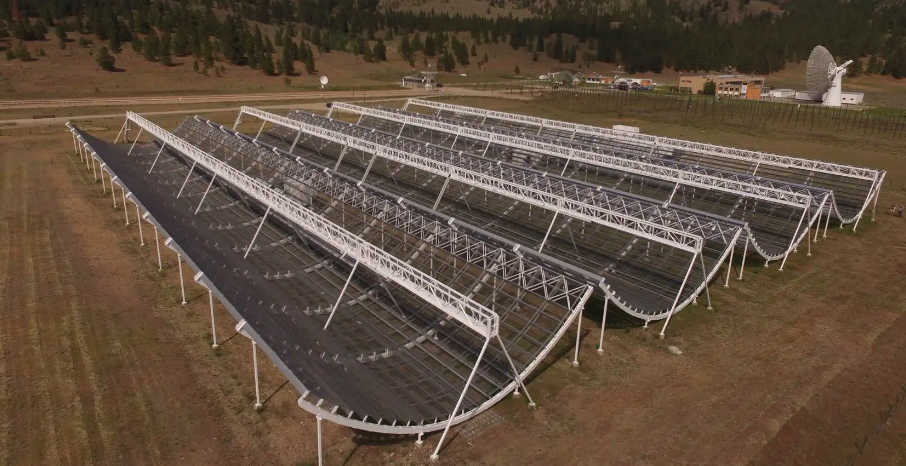
\includegraphics[width = 12cm]{img/chime.png}
% \caption{Telescopio experimental CHIME en Canada \cite{CHIME}.}
% \label{fig:chime}
% \end{figure}

% La figura \ref{fig:chime}, corresponde al telescopio experimental sin partes móviles, sintonizado para observar Hidrógeno y con un correlacionador capaz generar una apertura sintética para encontrar fenómenos astrofísicos transitorios de radio. Trabaja con una arquitectura de instrumentos remotos.

% \subsection{Guía de Construcción de Radiotelescopio con una RTL-SDR}

% Un enfoque para hacer radioastronomía con componentes comerciales y de bajo costo. Se utilizan radios definidas por software como receptor de radiofrecuencia y destaca las herramientas y software para observar la línea de 21cm.

% \begin{figure}
% \centering
% 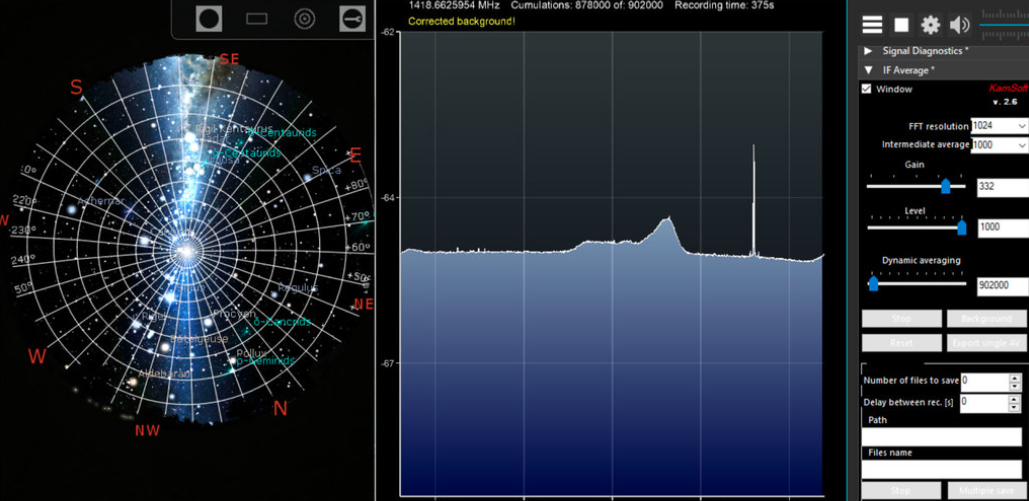
\includegraphics[width = 12cm]{img/rtlsdr.png}
% \caption{Software utilizado por RTL-SDR Blog para observar Hidrógeno neutro con una RTL-SDR\cite{RTLSDR2018}.}
% \label{fig:rtl}
% \end{figure}

% La figura \ref{fig:rtl}, corresponde al software de recepción de radio sintonizado en la frecuencia de emisión del hidrógeno neutro a la derecha, además del software de seguimiento astronómico y catalogo de objetos de interés.